\section{Discussion}
\subsection{Improving Boundary Conditions}
In chapter TODO we assumed that the boundary conditions were always lined up perfectly with the grid cells. We also assumed that the velocity of all solids were zero. If we would allow solids to have a velocity $\vec{u^{solid}}$, Equation \ref{TODO} has to be changed to

\begin{equation}
u^{solid}_{i+1/2,j}  = {u^*}_{i+1/2,j} - \frac{\Delta t }{\rho}\frac{p_{i+1,j} - p_{i,j}}{\Delta x}
\end{equation}

%\noident
The more complicated case when setting up the pressure equations is when a cell is only partially covered with solid or air. Figure \ref{boundarycases} shows two different cases, one that our simple approach covers very well and one that would lead to rectangular artifacts.

\begin{figure}[ht!]
\centering
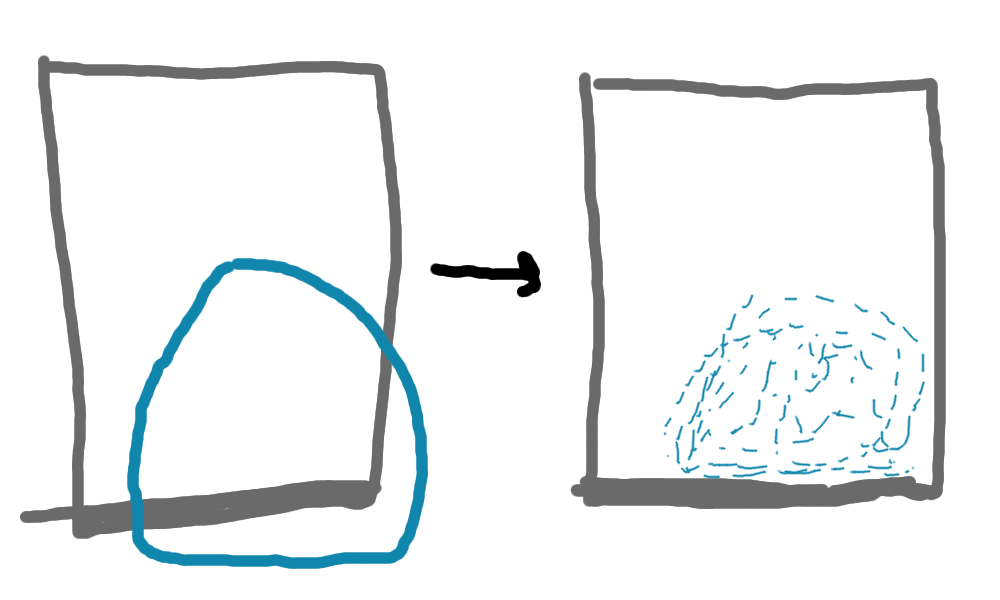
\includegraphics[width=80mm]{ch3/create.png}
\caption{A simple caption}
\label{boundarycases}
\end{figure}

Batty et al [2] presented a way to deal with irregular boundary geometry. It would be interesting to apply their ideas to the fluid multigrid solver in this thesis. When setting up the pressure equations, we would need a way to find out how much of a cell is covered by fluid. Even more specific, how much of the area nearby an edge is covered by fluid? The only change we would have to make would be in Equation \ref{pressureeq}. If $m$ is the previously mentioned fluid cover function ($0 \leq m \leq 1$), our linear system of equations need to satisfy the following:

\begin{equation}
\begin{split}
(m_{i-1/2,j} + m_{i+1/2,j} + m_{i,j-1/2} + m_{i,j+1/2})p_{i,j} - \\ 
m_{i-1/2,j} p_{i-1,j} - 
m_{i+1/2,j}p_{i+1,j} & - \\
m_{i,j-1/2}p_{i,j-1} - 
m_{i,j+1/2}p_{i,j+1} = \\ 
-\frac{\rho \Delta x}{\Delta t}(m_{i+1/2,j}{u^*}_{i+1/2,j} - m_{i-1/2,j}{u^*}_{i-1/2,j} + \\
m_{i,j+1/2}{v^*}_{i,j+1/2} - m_{i,j-1/2} {v^*}_{i,j-1/2})
\end{split}
\label{pressureeqvariational}
\end{equation}

\subsection{Advecting the Level Set}

We are constantly redefining the surface each step based on the position of the particles. This can lead to a noisy surface tracking. Another option that would be interesting to try would be to create a smooth level set once and then advect the level set. The free surface, where $\phi = 0$ should be advected with the fluid velocity and we need to solve Equation \ref{advectlevelset}.

\begin{equation}
\frac{\partial \phi}{\partial t} + \nabla \phi \cdot \vec{u} = 0
\label{advectlevelset}
\end{equation}

Fedkiw and Osher[TODO] introduced high-order methods for solving Equation \ref{advectlevelset}. If we advect both the level set and all particles every substep there will be cases where particles exists in regions where $\phi > 0$. What to do with those particles is not clear. One option would be to only advect the escaped particles in the extrapolated velocity field and not let them affect the pressure solve.

\subsection{Parallel implementation}

Solving for pressure is the largest and the most computational expensive part of the FLIP algorithm. Most fluid simulators have traditionally been using a preconditioned conjugate gradient pressure solver. A very popular preconditioner to use is the Incomplete Cholesky Factorization. Although making the conjugate gradient method to converge faster, this preconditioner cn not be run in parallell which is unfortunate since one has to apply the preconditioner before every conjugate gradient step. The multigrid approach has the big advantage that every step is easy to port from a serial implementation to a parallel one. Given a grid size of $N_x$ and $N_y$, one can simply divide the grid into subregions proportional to the number of cores present on the arcitechure performing the computations. One of the benefits using the Red and Black Gauss-Seidel iteration scheme presented in Chapter TODO is that it does not matter in which order the subregions are updated in an iteration step since we are guaranteed that all neighboring cells had their values updated in previous step. The restriction and prolongation operators are also easy to perform in parallel since there are no read/write conflicts and once again the grid can be divided into subregions for each core available. Other trivial steps to run in parallel out of the items presented in the outline of the algorithm in Chapter TODO is:

\begin{enumerate}
\item Mark cells fluid
\item Apply external forces to grid
\item Create Level Set
\item Tranfser grid velocities to particles
\item Advect particles
\end{enumerate}

Transfering the particle velocities to the grid is harder to run in parallel because of the fact that two particles could potentially be writing to the same velocity in the grid at the same time and therefore introduce a write condition. This motivates us to use a special data structure for particles, storing them in different banks depending on their spatial position. Similar to the Red and Black Gauss-Seidel, we only update regions in parallel that are not neighbors and we can therefore assume that inside a thread there will never be a write condition.
\newline
\newline
Reinitializing the level set and extrapolating velocites outside of the fluid region are also a bit more complicated since these steps are both using the fast sweeping method. In [TODO] explains an algorithm that solves the Eiokonal equation in parallel using a fast sweeping approach. Similar method can be used to extrapolate the velocities as well.
